\documentclass[12pt, a4paper]{article}

\usepackage{amsmath}
\usepackage{graphicx}
%\usepackage{setspace}
%\usepackage[cm]{fullpage}
\usepackage{a4wide}
\usepackage[colorlinks, breaklinks=true, bookmarks=true]{hyperref}

%\doublespacing

%\let\WriteBookmarks\relax

% functions and operations that shouldn't be in Italic font:
\newcommand{\sech}{\mathrm{sech}}
\newcommand{\Real}{\mathrm{Re}}
\newcommand{\Imag}{\mathrm{Im}}
\newcommand{\Tr}{\mathrm{Tr}}

% derivatives:

\newcommand{\deriv}[2]{\frac{d#1}{d#2}}
\newcommand{\nderiv}[3]{\frac{d^#3#1}{{d#2}^#3}}
\newcommand{\pderiv}[2]{\frac{\partial#1}{\partial#2}}
% 2'nd partial derivatives:
\newcommand{\spderiv}[2]{\frac{\partial^2#1}{{\partial#2}^2}}
\newcommand{\pderivdd}[3]{\frac{\partial^2#1}{\partial#2\partial#3}}
% functional derivatives:
\newcommand{\fnlderiv}[2]{\frac{\delta#1}{\delta#2}}
\newcommand{\fnlderivdd}[3]{\frac{\delta^2#1}{\delta#2\delta#3}}

% small matrix:
\newenvironment{bsmatrix}{\left[\begin{smallmatrix}}{\end{smallmatrix}\right]}

% big 0 in a matrix:
\newcommand{\BigFig}[1]{\parbox{12pt}{\Huge #1}}
\newcommand{\BigZero}{\BigFig{0}}
\newcommand{\ket}[1]{\left|#1\right>}
\newcommand{\bra}[1]{\left<#1\right|}
% an eighenstate:
\newcommand{\eigs}[1]{\left|\varphi_{#1}\right>}
% brackets with operator:
\newcommand{\bracketsO}[3]{\left<#1 \left|#2 \right|#3 \right>}
% with a bigger |:
\newcommand{\bracketsObigm}[3]{\left<#1\! \bigm|\!#2 \!\bigm|\!#3 \right>}
% with the biggest |:
\newcommand{\bracketsObiggm}[3]{\left<#1\! \biggm|\!#2 \!\biggm|\!#3 \right>}
% brackets without operator:
\newcommand{\brackets}[2]{\left<#1 | #2\right>}
% with a bigger |:
\newcommand{\bracketsbigm}[2]{\left<#1 \bigm| #2\right>}
% with the biggest |:
\newcommand{\bracketsbiggm}[2]{\left<#1 \biggm| #2\right>}
% expectation value:
\newcommand{\exval}[1]{\left<#1 \right>}
% bold operator:
\newcommand{\operator}[1]{\mathbf{\hat#1}}
% commutation relation:
\newcommand{\commut}[2]{\left[#1, #2\right]}

\newcommand{\etal}{\textit{et al.}\ }
\newcommand{\ie}{i.\,e.\ }
\newcommand{\eg}{e.\,g.\ }

\begin{document}
\title{Propagator for a stationary Hamiltonian\\
Computational project No. 3}
\author{Ido Schaefer}
\date{\today}
\maketitle

A general remark: Atomic units are used throughout.

\section{Algorithm}

The propagator is based on the computation of the operation of the evolution operator of a stationary system,
\[
	\operator{U}(t, 0) = \exp\left(-i\operator{H}t\right)
\]
on the initial state, $\ket{\psi_0}$. The operation of the function of matrix is computed by a Newton interpolation in Leja points. The algorithm is implemented in the function \texttt{fMtLeja.m}.

The computational process ends when the estimated error is smaller than a user defined tolerance parameter, which will be denoted by $\tau$. The error of an $n$ point expansion is estimated by:
\begin{equation}\label{eq:Eest}
	\epsilon_{est,n} \equiv |a_n| \Vert(\operator{H}-x_0)(\operator{H}-x_1)\cdots(\operator{H}-x_n)\ket{\psi_0}\Vert
\end{equation}
where $x_n$ is the last Leja point used in the interpolation. This replaces the more accurate estimation by the norm of the expression for the next term in the expansion:
\begin{equation}
	|a_{n+1}| \Vert(\operator{H}-x_0)(\operator{H}-x_1)\cdots(\operator{H}-x_n)\ket{\psi_0}\Vert
\end{equation}
(I learned it from a program written by Hillel).

\section{Application}

The algorithm is tested on two simple systems in which an analytic solution is available. Then it is applied to a Morse potential oscillator. We demonstrate that the Bohr frequencies of the system can be extracted from the dynamics of the system, as solved by the algorithm.

\subsection{Two level system}
The first test system is a two level system. Hamiltonian of the two level system is:
\begin{equation}
	\operator{H} =
	\begin{bmatrix}
		1 & 1 \\
		1 & 1
	\end{bmatrix}
\end{equation}
Let us define:
\begin{align}
	\ket{1} &\equiv
	\begin{bmatrix}
		1  \\
		0	
	\end{bmatrix} \label{eq:state1}\\ 
	\ket{2} &\equiv
	\begin{bmatrix}
		0  \\
		1	
	\end{bmatrix} \label{eq:state2}
\end{align}
The initial state is:
\begin{equation*}
	\ket{\psi_0} = \ket{1}
\end{equation*}

The occupation numbers of the states~\eqref{eq:state1}, \eqref{eq:state2}, perform Rabbi oscillations in the frequency $\omega=2_{a.u.}$. For the given initial state, we have:
\begin{equation}\label{eq:TLSanal}
	\brackets{2}{\psi(t)} = \sin^2(t)
\end{equation}

The algorithm is tested on this system in the procedure \texttt{testLejaTLS.m}. The solution is computed in 100 equally spaced time points, where the final time is $T=10_{a.u.}$. The tolerance parameter is chosen to be $\tau=10^{-8}$. The resulting time-dependent occupation numbers are plotted in Fig.~\ref{fig:TLS}. 

\begin{figure}[htb]
	\centering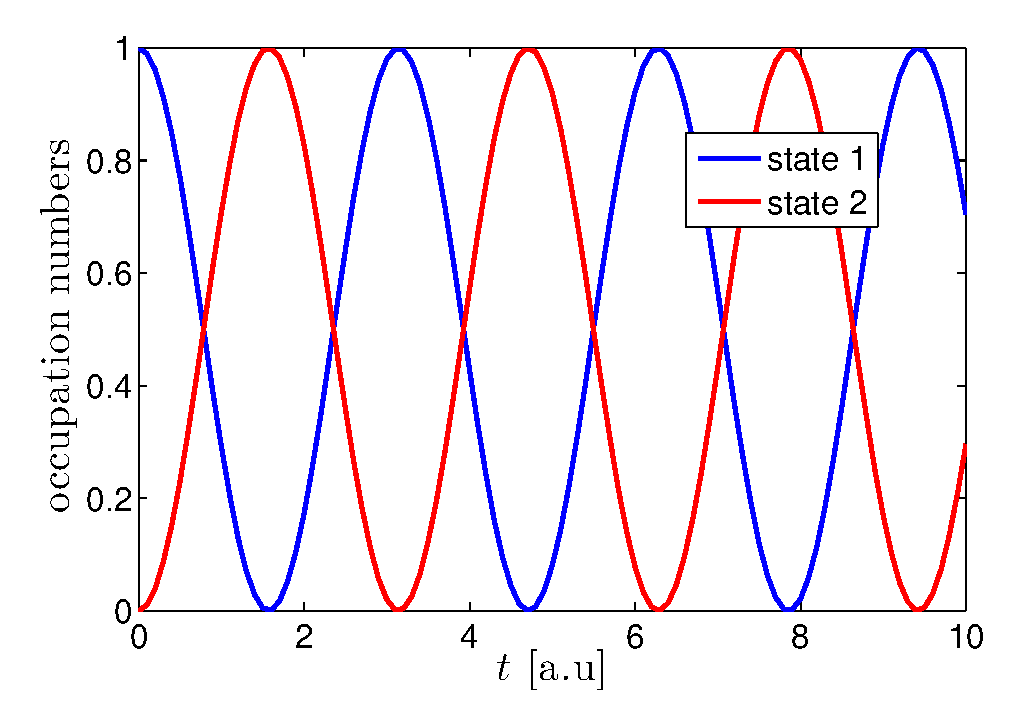
\includegraphics[width=3in]{TLSoc}
	\caption{The occupation numbers in the two level system Vs.\ $t$.}\label{fig:TLS}
\end{figure}

The deviation from the analytic result, \eqref{eq:TLSanal}, is computed in all time points. The maximal deviation is $3.1994\times10^{-9}$. The maximal estimated error of the solution by Eq.~\eqref{eq:Eest} is $8.9276\times10^{-9}$. Eq.~\eqref{eq:Eest} is shown to be a reasonable estimation for the order of magnitude of the error.

\subsection{Harmonic oscillator}
The second test system is a one dimensional harmonic oscillator, with mass $m=1_{a.u.}$ and characteristic frequency $\omega_0=1_{a.u.}$. The Hamiltonian is:
\begin{equation}
	\operator{H} = \frac{\operator{P}^2}{2} + \frac{\operator{X}^2}{2}
\end{equation}
Let us denote the ground state by $\ket{\varphi_0}$; the initial state is:
\begin{equation}
	\ket{\psi_0} = \exp\left(i 8 \operator{X}\right)\ket{\varphi_0}
\end{equation}
This initial state is a coherent state. Hence, $\exval{\operator{X}}$ evolves in time like the $x$ coordinate of the classical system with the corresponding classical Hamiltonian, and initial momentum $p=8_{a.u.}$. Thus:
\begin{equation}\label{eq:Harmonicanal}
	\exval{\operator{X}}(t) = 8\sin(t)
\end{equation}

The propagation of the system is implemented in the procedure \texttt{testLejaHarmonic.m}. We use an $x$ grid of $N_x=128$ equally spaced points. The $x$ domain, \text{$[x_{min},\, x_{max}]$}, and the spacing between neighbouring grid points, $\Delta x$, are chosen as to satisfy the following requirements:
\begin{align}
	& K_{max} = V_{max} \label{eq:gcond1} \\
	& V(x_{min}) = V(x_{max}) \label{eq:gcond2}
\end{align}
where $K_{max}$ and $V_{max}$ are the maximal kinetic and potential energies in the corresponding classical system. These requirements, together with the chosen $N_x$, determine the grid uniquely. The resulting $x$ domain is \text{$[-8\sqrt{\pi},\, 8\sqrt{\pi})$}.

The Hamiltonian operation is approximated by the Fourier grid method in the function \texttt{Hpsi.m}.

Here, again, the solution is computed in 100 equally spaced time points, with $T=10_{a.u.}$. The tolerance parameter is chosen to be $\tau=10^{-10}$. The resulting $\exval{\operator{X}}(t)$ is plotted in Fig.~\ref{fig:Harmonic}.

\begin{figure}[htb]
	\centering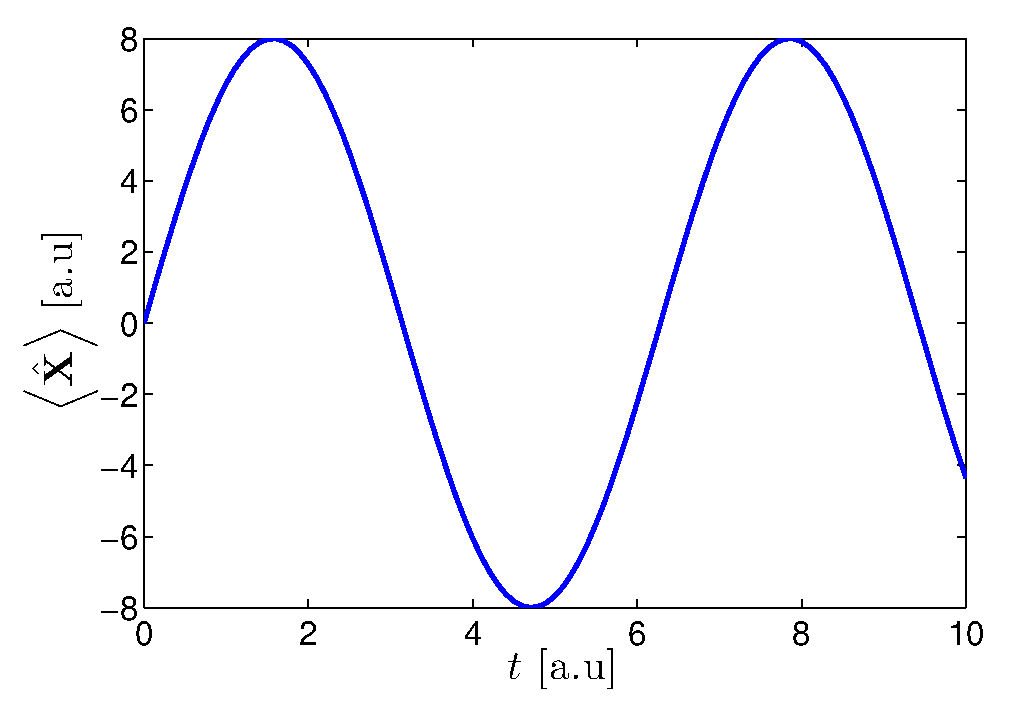
\includegraphics[width=3in]{harmonicmx}
	\caption{$\exval{\operator{X}}(t)$ Vs.\ $t$, for the Harmonic oscillator system.}\label{fig:Harmonic}
\end{figure}

The deviation from the analytic result in \eqref{eq:Harmonicanal} is computed in all time points. The maximal deviation is \text{$1.7347\times10^{-10}$}. The maximal estimated error of $\ket{\psi(t)}$ is \text{$9.2352\times10^{-11}$}. Eq.~\eqref{eq:Eest} is shown again to be successful in estimating the order of magnitude of the error.

\subsection{Bohr frequencies of a Morse potential oscillator}
The algorithm is applied to a one-dimensional particle with $m=1_{a.u.}$ in a Morse potential:
\begin{equation}\label{eq:Morse}
	V_{M}(x) = D_0[\exp(-a x) - 1]^2.
\end{equation}
We choose: $a=0.2$, $D_0 = 12.5$. The parameters are chosen as to satisfy:
\[
	\nderiv{V_{M}(x)}{x}{2} = 1_{a.u.}.
\]
 
The Hamiltonian is:
\begin{equation}
	\operator{H} = \frac{\operator{P}^2}{2} + V_{M}\left(\operator{X}\right)
\end{equation}
The initial state is:
\begin{equation}\label{eq:psi0Morse}
	\ket{\psi_0} = \exp\left(i 0.5 \operator{X}\right)\ket{\varphi_0}
\end{equation}
where $\ket{\varphi_0}$ denotes the ground state of the system.

The system in study is a nonlinear oscillator. In the harmonic oscillator system, the $\exval{\operator{X}}(t)$ spectrum consists only of the characteristic frequency of the oscillator. Here, we expect to see in the $\exval{\operator{X}}(t)$ spectrum nonlinear effects, like the appearance of overtone frequencies. The spectral analysis of $\exval{\operator{X}}(t)$ can be used to extract some of the Bohr frequencies of the system:
\[
	\omega_{n,m} = \frac{E_n - E_m}{\hbar}
\]
from the system's dynamics.

If we used a Fourier analysis for this purpose, a very long propagation time would have been required. Hence, we use the Krylov Basis Diagonalization Method (KBDM) instead. This method constitutes the basis for one of the approaches to Filter Diagonalization  \cite{FDM}. Let us denote a time signal by $c(t)$. In KBDM, a set of $N_\omega$ complex amplitudes, $A_k$, and frequencies, $\omega_k$, are fitted to a parametric representation of the signal:
\begin{equation}
	c(t) = \sum_{k=1}^{N_\omega}A_k \exp(-i\omega_k t)
\end{equation}
The problem is formulated by the means of linear algebra. Experience shows that this method can often give impressive results when used to reproduce the spectrum of a signal. Unfortunately, occasionally it tends to be rather unstable numerically. In addition, it often fails in the separation of similar frequencies (maybe because the problem itself is ill defined in such a case).

The whole process is implemented in the procedure \texttt{LejaMorse.m}. The $x$ grid consists of $N_x=32$ equally spaced points. It is chosen as to satisfy the conditions \eqref{eq:gcond1}, \eqref{eq:gcond2}. The two conditions constitute a nonlinear system of equations. It is solved in the procedure \texttt{nlgrid.m}. The potential in the resulting grid is plotted in Fig.~\ref{fig:VMorse}.

\begin{figure}[htb]
	\centering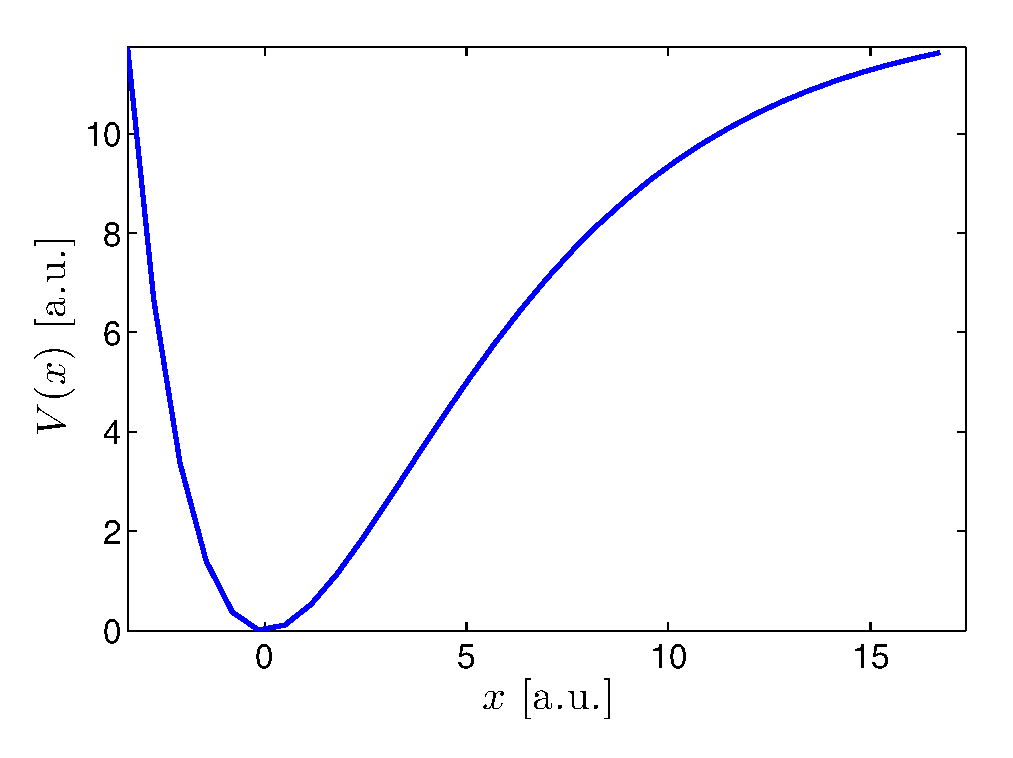
\includegraphics[width=3in]{morseV}
	\caption{The Morse potential in the chosen $x$ grid.}\label{fig:VMorse}
\end{figure}

The Hamiltonian operation is performed by the Fourier grid method.

The ground state is computed by the diagonalization of the Hamiltonian in the function \texttt{gsV.m}. In order to check the reliability of the approximation by the discretized grid, the resulting eigenenergies are compared to the analytic result:
\begin{equation}\label{eq:Emorse}
	E_n = D_0 - \frac{a^2\hbar^2}{2m}\left(\frac{\sqrt{2mD_0}}{a\hbar} - n - \frac{1}{2} \right)
\end{equation}
Let us define the relative error of the computed eigenenergies $E_{n,num}$ from the analytic eigenenergies $E_{n,anal}$:
\begin{equation}
	\epsilon_{rel,n} = \left| \frac{E_{n,num}-E_{n,anal}}{E_{n,anal}}\right|
\end{equation}
In Fig.~\ref{fig:epsMorse}, $\log_{10}(\epsilon_{rel})$ is plotted Vs.\ $n$. It is shown that the discretization error is not large, at least for the lower energy eigenstates. The initial momentum given to the ground state in \eqref{eq:psi0Morse} is not large, so we remain in the lower eigenstate regime. Thus, the approximation can be considered quite accurate.

\begin{figure}[htb]
	\centering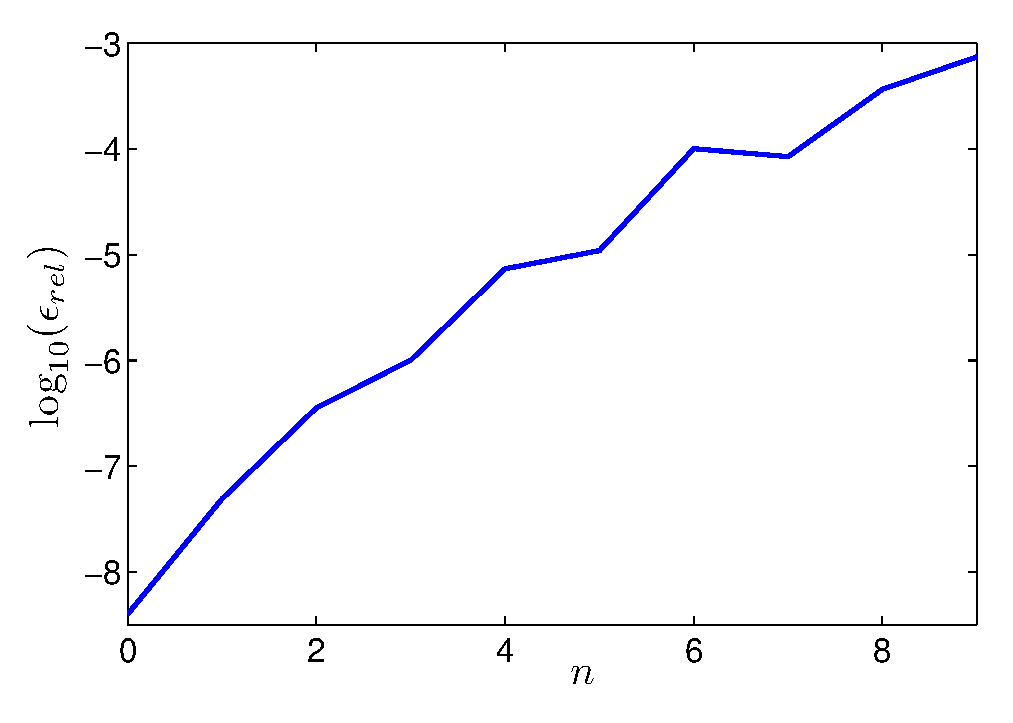
\includegraphics[width=3in]{morseEerror}
	\caption{$\log_{10}(\epsilon_{rel})$ Vs.\ $n$ for the Morse potential system.}\label{fig:epsMorse}
\end{figure}

The solution is computed in 1000 equally spaced time points, with $T=100_{a.u.}$. An extremely small tolerance parameter is chosen, $\tau = 10^{-13}$. It was found that a highly accurate solution is required, because the Bohr frequencies $\omega_{n+1,n}$ for different $n$ values are very close to each other. Consequently, the separation ability of the KBDM is quite limited for these frequencies, and it is very sensitive to noises.

$\exval{\operator{X}}(t)$ is computed in all time points. The KBDM analysis of the resulting signal is performed in the procedure \texttt{FBDMrinp.m}, adjusted for a real signal. We deal only with the 15 frequencies with the largest amplitudes. The resulting spectrum is plotted in Fig.~\ref{fig:spectrum}. It can be inspected that the resulting frequencies are divided into 4 groups of different harmonics:
\begin{equation}\label{eq:wl}
	\omega_{n+l,n}, \qquad\qquad l=1,2,3,4
\end{equation}
The resulting frequencies can be assigned to different $n$ and $l$ values by inspection.

\begin{figure}[htb]
	\centering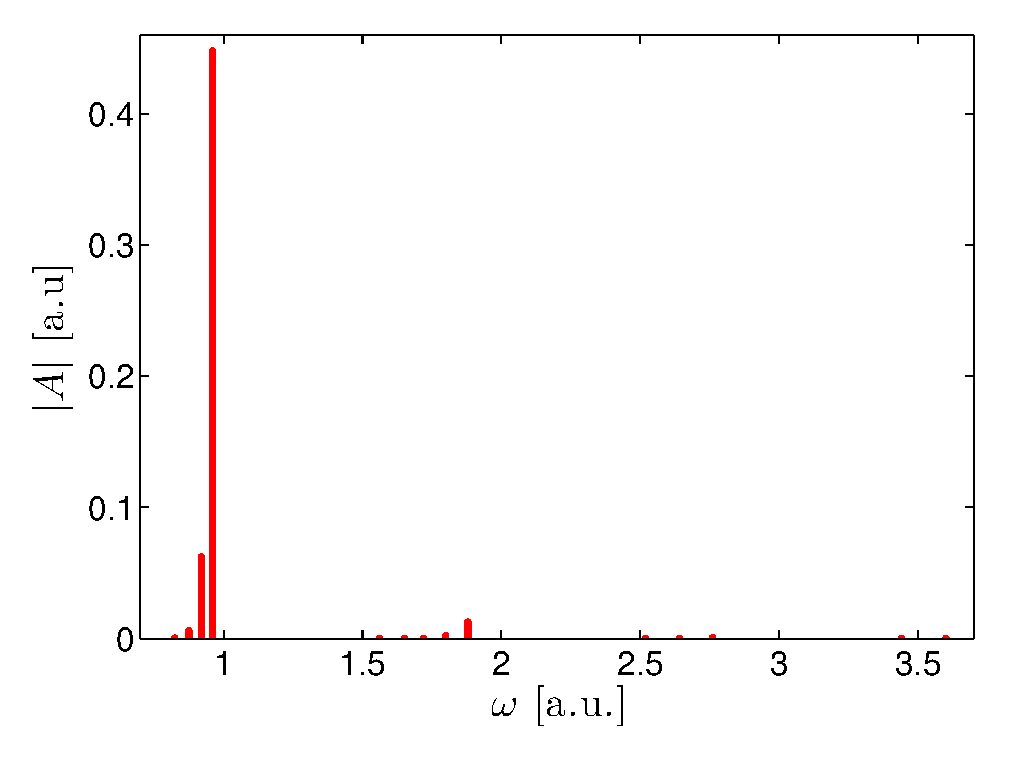
\includegraphics[width=3in]{morse_omega}
	\caption{The $\exval{\operator{X}}(t)$ spectrum for the Morse potential system. The absolute values of the 15 largest amplitudes in the line list are plotted Vs.\ $\omega$.}\label{fig:spectrum}
\end{figure}

In Table~\ref{tab}, the resulting frequencies are compared to the assigned Bohr frequencies of the system, computed from the eigenenergies obtained by diagonalization of the Hamiltonian. The relative error is defined as:
\begin{equation}
	\epsilon_\omega = \left| \frac{\omega_{KBDM} - \omega_{diag}}{\omega_{diag}} \right|
\end{equation}
where $\omega_{KBDM}$ is the frequency obtained by the spectral analysis of $\exval{\operator{X}}(t)$, and $\omega_{diag}$ is the corresponding Bohr frequency computed by diagonalization. The frequencies are sorted into 4 groups characterized by the $l$ values from Eq.~\eqref{eq:wl}. The KBDM method fails in the separation of the lower frequencies in the system, which are too similar. These cannot be assigned to a distinct Bohr frequency, but only to an $l$ value. However, it is very successful in computing most of the Bohr frequencies, which are obtained with high accuracy.

It is demonstrated that the energy level structure of the system can be deduced from the dynamics, as computed by the algorithm. 

\begin{table}
\begin{center}
\renewcommand{\arraystretch}{1.2}
\begin{tabular}{|c||c|c|c|}	\hline
	$l$ & $\omega_{KBDM}$ [a.u.] & \textbf{Bohr frequency assignment} & $\epsilon_{\omega}$\\ \hline \hline
	1 & 0.82438 & --- & --- \\ \cline{2-4}
	  & 0.87498 & --- & --- \\ \cline{2-4}
	  & 0.87572 & $\omega_{3,2}$ & $4.8646\times 10^{-3}$ \\ \cline{2-4}
	  & 0.92026 & $\omega_{2,1}$ & $2.8838\times 10^{-4}$ \\ \cline{2-4}
	  & 0.96000 & $\omega_{1,0}$ & $1.2548\times 10^{-6}$ \\ \hline \hline
	2 & 1.5608 & $\omega_{6,4}$ & $9.2135\times 10^{-4}$ \\ \cline{2-4}
	  & 1.6521 & $\omega_{5,3}$ & $7.4070\times 10^{-3}$ \\ \cline{2-4}
	  & 1.7194 & $\omega_{4,2}$ & $3.7693\times 10^{-4}$ \\ \cline{2-4}
	  & 1.8000 & $\omega_{3,1}$ & $1.2929\times 10^{-5}$ \\ \cline{2-4}
	  & 1.8800 & $\omega_{2,0}$ & $6.1639\times 10^{-7}$ \\ \hline \hline
	3 & 2.5198 & $\omega_{5,2}$ & $6.0794\times 10^{-5}$ \\ \cline{2-4}
  	  & 2.6400 & $\omega_{4,1}$ & $4.8719\times 10^{-6}$ \\ \cline{2-4}
	  & 2.7600 & $\omega_{3,0}$ & $5.3368\times 10^{-7}$ \\ \hline \hline
  	4 & 3.4400 & $\omega_{5,1}$ & $1.3658\times 10^{-6}$ \\ \cline{2-4}
  	  & 3.6000 & $\omega_{4,0}$ & $1.5497\times 10^{-7}$ \\ \hline 
\end{tabular}
\end{center}
\caption{Assignment of the resulting frequencies to the Bohr frequencies of the Morse potential system, and the relative deviation of the resulting frequencies from the Bohr frequencies computed by direct diagonlization.}\label{tab}
\end{table}


\begin{thebibliography}{999}
\bibitem{FDM}
	V. A. Mandelshtam, \emph{``FDM: the filter diagonalization method for data processing in NMR experiments"}, Progress in Nuclear Magnetic Resonance Spectroscopy, 38 (2001)
\end{thebibliography}


\end{document}